

\tikzset{every picture/.style={line width=0.75pt}} %set default line width to 0.75pt        

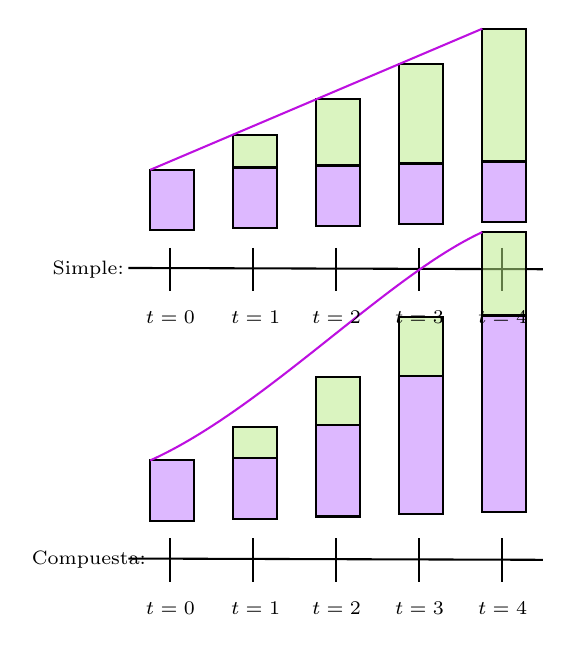
\begin{tikzpicture}[x=0.75pt,y=0.75pt,yscale=-1,xscale=1]
%uncomment if require: \path (0,300); %set diagram left start at 0, and has height of 300

%============ CAPITALIZACIÓN SIMPLE (TOP) ============
%Straight Lines [id:da001] - Main timeline (simple)
\draw    (203,140) -- (402.68,140.61) ;
%Straight Lines [id:da002] - Vertical ticks (simple)
\draw    (223.2,130.27) -- (223.2,151.27) ;
\draw    (263.2,130.27) -- (263.2,151.27) ;
\draw    (303.2,130.27) -- (303.2,151.27) ;
\draw    (343.2,130.27) -- (343.2,151.27) ;
\draw    (383.2,130.27) -- (383.2,151.27) ;

%Stacked rectangles for simple interest (t=0)
\draw  [fill={rgb, 255:red, 144; green, 19; blue, 254 }  ,fill opacity=0.3 ] (213.53,92.73) -- (234.81,92.73) -- (234.81,121.73) -- (213.53,121.73) -- cycle ;
%Stacked rectangles for simple interest (t=1)
\draw  [fill={rgb, 255:red, 144; green, 19; blue, 254 }  ,fill opacity=0.3 ] (253.53,91.73) -- (274.81,91.73) -- (274.81,120.73) -- (253.53,120.73) -- cycle ;
\draw  [fill={rgb, 255:red, 184; green, 233; blue, 134 }  ,fill opacity=0.52 ] (253.53,75.73) -- (274.81,75.73) -- (274.81,91.53) -- (253.53,91.53) -- cycle ;
%Stacked rectangles for simple interest (t=2)
\draw  [fill={rgb, 255:red, 144; green, 19; blue, 254 }  ,fill opacity=0.3 ] (293.53,90.73) -- (314.81,90.73) -- (314.81,119.73) -- (293.53,119.73) -- cycle ;
\draw  [fill={rgb, 255:red, 184; green, 233; blue, 134 }  ,fill opacity=0.52 ] (293.53,58.73) -- (314.81,58.73) -- (314.81,90.53) -- (293.53,90.53) -- cycle ;
%Stacked rectangles for simple interest (t=3)
\draw  [fill={rgb, 255:red, 144; green, 19; blue, 254 }  ,fill opacity=0.3 ] (333.53,89.73) -- (354.81,89.73) -- (354.81,118.73) -- (333.53,118.73) -- cycle ;
\draw  [fill={rgb, 255:red, 184; green, 233; blue, 134 }  ,fill opacity=0.52 ] (333.53,41.73) -- (354.81,41.73) -- (354.81,89.53) -- (333.53,89.53) -- cycle ;
%Stacked rectangles for simple interest (t=4)
\draw  [fill={rgb, 255:red, 144; green, 19; blue, 254 }  ,fill opacity=0.3 ] (373.53,88.73) -- (394.81,88.73) -- (394.81,117.73) -- (373.53,117.73) -- cycle ;
\draw  [fill={rgb, 255:red, 184; green, 233; blue, 134 }  ,fill opacity=0.52 ] (373.53,24.73) -- (394.81,24.73) -- (394.81,88.53) -- (373.53,88.53) -- cycle ;

%============ CAPITALIZACIÓN COMPUESTA (BOTTOM) ============
%Straight Lines [id:da003] - Main timeline (compound)
\draw    (203,280) -- (402.68,280.61) ;
%Straight Lines [id:da004] - Vertical ticks (compound)
\draw    (223.2,270.27) -- (223.2,291.27) ;
\draw    (263.2,270.27) -- (263.2,291.27) ;
\draw    (303.2,270.27) -- (303.2,291.27) ;
\draw    (343.2,270.27) -- (343.2,291.27) ;
\draw    (383.2,270.27) -- (383.2,291.27) ;

%Stacked rectangles for compound interest (t=0)
\draw  [fill={rgb, 255:red, 144; green, 19; blue, 254 }  ,fill opacity=0.3 ] (213.53,232.73) -- (234.81,232.73) -- (234.81,261.73) -- (213.53,261.73) -- cycle ;
%Stacked rectangles for compound interest (t=1)
\draw  [fill={rgb, 255:red, 144; green, 19; blue, 254 }  ,fill opacity=0.3 ] (253.53,231.73) -- (274.81,231.73) -- (274.81,260.73) -- (253.53,260.73) -- cycle ;
\draw  [fill={rgb, 255:red, 184; green, 233; blue, 134 }  ,fill opacity=0.52 ] (253.53,216.8) -- (274.81,216.8) -- (274.81,231.53) -- (253.53,231.53) -- cycle ;
%Stacked rectangles for compound interest (t=2)
\draw  [fill={rgb, 255:red, 144; green, 19; blue, 254 }  ,fill opacity=0.3 ] (293.53,215.73) -- (314.81,215.73) -- (314.81,259.73) -- (293.53,259.73) -- cycle ;
\draw  [fill={rgb, 255:red, 184; green, 233; blue, 134 }  ,fill opacity=0.52 ] (293.53,192.73) -- (314.81,192.73) -- (314.81,215.53) -- (293.53,215.53) -- cycle ;
%Stacked rectangles for compound interest (t=3)
\draw  [fill={rgb, 255:red, 144; green, 19; blue, 254 }  ,fill opacity=0.3 ] (333.53,191.97) -- (354.81,191.97) -- (354.81,258.73) -- (333.53,258.73) -- cycle ;
\draw  [fill={rgb, 255:red, 184; green, 233; blue, 134 }  ,fill opacity=0.52 ] (333.53,163.41) -- (354.81,163.41) -- (354.81,191.97) -- (333.53,191.97) -- cycle ;
%Stacked rectangles for compound interest (t=4)
\draw  [fill={rgb, 255:red, 144; green, 19; blue, 254 }  ,fill opacity=0.3 ] (373.53,162.97) -- (394.81,162.97) -- (394.81,257.73) -- (373.53,257.73) -- cycle ;
\draw  [fill={rgb, 255:red, 184; green, 233; blue, 134 }  ,fill opacity=0.52 ] (373.53,122.74) -- (394.81,122.74) -- (394.81,162.53) -- (373.53,162.53) -- cycle ;

%Straight Lines [id:da005] - Growth line (simple)
\draw [color={rgb, 255:red, 189; green, 16; blue, 224 }  ,draw opacity=1 ]   (213.53,92.73) -- (373.53,24.73) ;
%Curve Lines [id:da006] - Growth curve (compound)
\draw [color={rgb, 255:red, 189; green, 16; blue, 224 }  ,draw opacity=1 ]   (213.53,232.73) .. controls (268.66,207.85) and (327.66,143.85) .. (373.53,122.74) ;

% Text Node - Time labels (simple - top)
\draw (210,159.4) node [anchor=north west][inner sep=0.75pt]  [font=\scriptsize]  {$t=0$};
\draw (251,159.4) node [anchor=north west][inner sep=0.75pt]  [font=\scriptsize]  {$t=1$};
\draw (290,159.4) node [anchor=north west][inner sep=0.75pt]  [font=\scriptsize]  {$t=2$};
\draw (330,159.4) node [anchor=north west][inner sep=0.75pt]  [font=\scriptsize]  {$t=3$};
\draw (370,159.4) node [anchor=north west][inner sep=0.75pt]  [font=\scriptsize]  {$t=4$};

% Text Node - Time labels (compound - bottom)
\draw (210,299.4) node [anchor=north west][inner sep=0.75pt]  [font=\scriptsize]  {$t=0$};
\draw (251,299.4) node [anchor=north west][inner sep=0.75pt]  [font=\scriptsize]  {$t=1$};
\draw (290,299.4) node [anchor=north west][inner sep=0.75pt]  [font=\scriptsize]  {$t=2$};
\draw (330,299.4) node [anchor=north west][inner sep=0.75pt]  [font=\scriptsize]  {$t=3$};
\draw (370,299.4) node [anchor=north west][inner sep=0.75pt]  [font=\scriptsize]  {$t=4$};

% Text Node - Labels
\draw (165,135) node [anchor=north west][inner sep=0.75pt]  [font=\scriptsize]  {Simple:};
\draw (155,275) node [anchor=north west][inner sep=0.75pt]  [font=\scriptsize]  {Compuesta:};


\end{tikzpicture}
